\subsection{Sub $6\unit{\giga\hertz}$ transceiver front-end in $22$-$\unit{\nano\meter}$ FD-SOI CMOS}

	The final article discussed, \cite{FDSOI2}, proposes a highly integrated sub-$6\unit{\giga\hertz}$ --specifically, $f_{\symup{RF}}\in \left[ 1.25\unit{\giga\hertz}, 5.5\unit{\giga\hertz} \right]$-- tranceiver (TRx) front-end for cellular base stations. The IC is fabricated using 22nm FD-SOI technology. In order to meet the application requirements while using on-chip power amplifiers, the authors chose to use a $12.5\unit{\ohm}$ impedance. The advantage of using a low impedance is that it allows for low-voltage power amplification, since $P_{\symup{diss}}={V^2}{Z^{-1}}$. However, low input impedance --in the Rx front-end-- reduces the input voltage; hence, the targeted noise figure is harder to reach and a higher supply voltage is needed for the LNA \cite{FDSOI2}. The proposed IC is shown in figure \ref{fig:FDSOI:TRX:system}.\par

	The integrated part of the transmitter (Tx) consists of two pre-power-amplifier (PPA1 and PPA2) stages with variable gain and a power amplifier (PA). Additionally, the RF input signal is translated to baseband, filtered through a low-pass filter (LPF) and it is translated again to $f_{\symup{RF}}$ before it is substracted from the output signal of the first pre-power-amplifier stage (PPA1); the LP filter is in parallel to PPA1 (see figure \ref{fig:FDSOI:TRX:system}). The LPF is necessary for suppressing any intermodulation products that occur from the RF digital to analog converter's (DAC) clock --preceding PPA1 and not shown in figure \ref{fig:FDSOI:TRX:system}-- and the signals \cite{FDSOI2}.

	The integrated part of the receiver (Rx) consists of a low noise amplifier (LNA), followed by a variable gain amplifier (VGA), a three-frequency-band equalizer and finally a buffer. There is also a switch connected to the antenna array used for enabling either the Tx or Rx.\par

	It is important to note that both the Rx and Tx feature no frequency translation (except for the LPF); hence, all the amplifiers require wide bandwidth. Finally, all amplifiers in figure \ref{fig:FDSOI:TRX:system} are fully differential.\par

	\begin{figure}[htb]
		\centering
		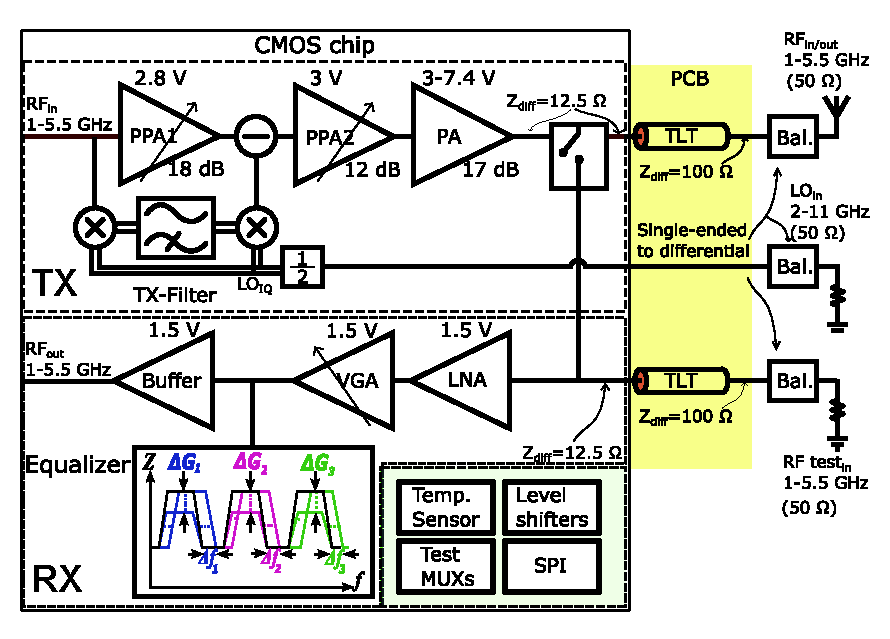
\includegraphics[width=\linewidth]{assets/FD-SOI/Sub_6GHz_TRX_assets/system.pdf}
			\caption{Simplified schematic of the proposed integrated tranceiver \cite{FDSOI2}.}
		\label{fig:FDSOI:TRX:system}
	\end{figure}

	\subsubsection{Noise factor} To better understand device-related noise, a means to quantify the device-added noise is needed. Let $G$ be the gain of an amplifier, $\symcal{S}_{\symup{in}}$, $\symcal{S}_{\symup{out}}$, $\symcal{N}_{\symup{in}}$ and $\symcal{N}_{\symup{out}}$ the power of the input signal, the power of the output signal, the power of the input noise and the power of the output noise, respectively. The ratio of the input SNR (signal-to-noise ratio), $\symup{SNR}_{\symup{in}}$, to the output SNR, $\symup{SNR}_{\symup{out}}$, is called \textsl{noise factor}.
	\begin{equation}
		\label{eq:noise_factor_definition}
		\symup{F}=\frac{\symup{SNR}_{\symup{in}}}{\symup{SNR}_{\symup{out}}}
	\end{equation}
	However, in practice \textsl{noise figure} is preferred over noise factor for characterizing a device. Noise figure, $\symup{NF}$, is the noise factor expressed in decibels; $\symup{NF}=10\log_{10}{\left(\symup{F}\right)}$ \cite{frenzel2015principles}.

	Some of the most prominent sources of device-added noise are resistors (thermal noise) and active devices \cite{RFICRogers}. We will prove that the noise factor of any real device is greater than unity. To do this we begin from the definition of noise factor in equation \eqref{eq:noise_factor_definition}.
	\begin{align*}
		& \symup{F} = \frac{\symup{SNR}_{\symup{in}}}{\symup{SNR}_{\symup{out}}} \Rightarrow\\
		& \symup{F} = \frac{\symcal{S}_{\symup{in}}}{\symcal{N}_{\symup{in}}} \cdot \frac{\symcal{N}_{\symup{out}}}{\symcal{S}_{\symup{out}}} \Rightarrow\\
		& \symup{F} = \frac{\symcal{S}_{\symup{in}}}{\symcal{N}_{\symup{in}}} \cdot \frac{G\cdot \symcal{N}_{\symup{in}} + \symcal{N}_{\symup{device}}}{G\symcal{S}_{\symup{in}}} \Rightarrow\\
		& \symup{F} = 1 + \frac{\symcal{N}_{\symup{device}}}{G\cdot \symcal{N}_{\symup{in}}} \gneqq 1,
	\end{align*}
	since $\symcal{N}_{\symup{device}}\gneqq 0$ for all real devices.

	\subsubsection{Low noise amplifier (LNA)}

		Low noise amplifiers (LNAs) are quite often the first component, after the antenna, in the Rx chain and that is because the noise figure/factor of the first subsystem dominates the system's total noise figure/factor \cite{frenzel2015principles}. This is apparent in the expression of the noise factor of system comprising of $N$ cascaded subsystems, each with gain $G_j$:
		\begin{equation}
			\label{eq:cascode_noise_factor}
			F_{\symup{tot}}=F_1+\sum_{i=2}^{N}{\frac{F_i-1}{\prod_{j=1}^{i-1}{G_j}}}
		\end{equation}

		\begin{figure}[ht!]
			\centering
			\begin{tikzpicture}
	% Paths, nodes and wires:
	\draw (-2.98, 3.27) -- (-2.48, 3.27);
	\draw (-1.5, -0.04) -- (-1.5, -0.29);
	\draw (1.5, -0.04) -- (1.5, -0.29);
	\path[draw={rgb,255:red,63;green,63;blue,63}, dash pattern={on 1.6pt off 1.6pt}, latex-latex] (-2.625, 1.21) -- (-0.75, 0.335);
	\node[nmos, arrowmos, xscale=-1](N1) at (-2.98, -0.04){} node[anchor=east] at (N1.text){$\symup{M}_{11}$};
	\node[nmos, arrowmos](N2) at (2.98, -0.04){} node[anchor=west] at (N2.text){$\symup{M}_{12}$};
	\node[nmos, arrowmos](N3) at (2.98, 2.5){} node[anchor=west] at (N3.text){$\symup{M}_{22}$};
	\node[nmos, arrowmos, xscale=-1](N4) at (-2.98, 2.5){} node[anchor=east] at (N4.text){$\symup{M}_{21}$};
	\draw (-2, 2.5) -- (2, 2.5);
	\node[vcc](N5) at (0, 4.5){} node[anchor=south] at ([yshift=-0.12cm]N5.text){$V_{\symup{DD}}$};
	\draw (-2, -0.04) to[cute inductor, inductors/width=1.5, inductors/coils=10, l_={$L_g$}] (2, -0.04);
	\node[ocirc](N6) at (-1.5, -0.29){} node[anchor=north] at ([yshift=0.04cm]N6.south){$v_{\symup{in}^{+}}$};
	\node[ocirc](N7) at (1.5, -0.29){} node[anchor=north] at ([yshift=0.04cm]N7.south){$v_{\symup{in}^{-}}$};
	\node[circ, yscale=-1] at (-0, 0.17){};
	\node[circ] at (-1.5, -0.04){};
	\node[circ] at (1.5, -0.04){};
	\draw (-0, -1.54) to[cute inductor, l={$L_{\symup{deg}}$}] (-0, -2.54);
	\draw (-2.98, -0.81) |- (-2.75, -1.29) -- (2.5, -1.29) -| (2.98, -0.81);
	\draw (-0, -1.54) -| (-0, -1.29);
	\node[circ] at (-0, -1.29){};
	\draw (-0, -2.54) -| (-0, -2.79);
	\node[tlground] at (-0, -2.79){};
	\node[tlground] at (-0, -2.79){};
	\draw (-2.98, 1.73) to[cute inductor, l_={$L_{dl}$}] (-2.98, 0.73);
	\node[circ, xscale=0.75, yscale=0.75] at (-2.625, 0.835){};
	\node[circ, xscale=0.75, yscale=0.75] at (-1.125, 0.335){};
	\draw (2.98, 0.73) to[cute inductor, l_={$L_{dr}$}] (2.98, 1.73);
	\node[circ, xscale=-0.75, yscale=-0.75] at (2.625, 1.625){};
	\path[draw={rgb,255:red,63;green,63;blue,63}, dash pattern={on 1.6pt off 1.6pt}, latex-latex] (-2.625, 1.585) -- (2.5, 1.585);
	\node[shape=rectangle, fill={rgb,255:red,255;green,255;blue,255}, minimum width=0.34cm, minimum height=0.235cm](N8) at (-0, 1.595){} node[anchor=center] at (N8.text){\textcolor{rgb,255:red,63;green,63;blue,63}{$k_2$}};
	\node[shape=rectangle, fill={rgb,255:red,255;green,255;blue,255}, minimum width=0.34cm, minimum height=0.34cm](N9) at (-1.688, 0.773){} node[anchor=center] at (N9.text){\textcolor{rgb,255:red,63;green,63;blue,63}{$k_1$}};
	\path[draw={rgb,255:red,63;green,63;blue,63}, dash pattern={on 1.6pt off 1.6pt}, latex-latex] (0.75, 0.335) -- (2.625, 1.21);
	\node[shape=rectangle, fill={rgb,255:red,255;green,255;blue,255}, minimum width=0.34cm, minimum height=0.34cm](N10) at (1.688, 0.773){} node[anchor=center] at (N10.text){\textcolor{rgb,255:red,63;green,63;blue,63}{$k_1$}};
	\node[ocirc](N11) at (-2.48, 3.27){} node[anchor=west] at ([xshift=-0.04cm]N11.east){$v_{\symup{out}^{-}}$};
	\node[circ] at (-2.98, 3.27){};
	\draw (2.48, 3.27) -- (2.98, 3.27);
	\node[ocirc](N12) at (2.48, 3.27){} node[anchor=east] at ([xshift=0.04cm]N12.west){$v_{\symup{out}^{+}}$};
	\node[circ] at (2.98, 3.27){};
	\draw (-1.25, 4.29) to[cute inductor, inductors/width=1.5, inductors/coils=10, l_={$L_{\symup{out}}$}] (1.25, 4.29);
	\draw (2.98, 3.27) |- (1.25, 4.29);
	\draw (-2.98, 3.27) |- (-1.25, 4.29);
	\node[circ] at (0, 4.5){};
	\node[circ] at (-0, 2.5){};
	\node[vcc](N13) at (-0, 0.17){} node[anchor=south] at ([yshift=-0.12cm]N13.text){$V_{\symup{CS}}$};
	\node[vcc](N14) at (0, 2.5){} node[anchor=south] at ([yshift=-0.12cm]N14.text){$V_{\symup{CG}}$};
\end{tikzpicture}
			\caption{LNA schematic with transformer feedback presented in \cite{FDSOI2}. $\symup{M}_{11}$ and $\symup{M}_{12}$ are identical. $\symup{M}_{21}$ and $\symup{M}_{22}$ are identical.}
			\label{fig:FDSOI:TRX:LNA}
		\end{figure}

		The noise factor of cascode MOSFET pair, where the transistor in common-source (CS) topology acts as the input transistor, is inversely proportional to the input transistor's transconductance, $g_{m,\symup{CS}}$, \cite{Adaptive2008}. Hence, the noise factor can be reduced by increasing the input transconductance \cite{FDSOI2} \cite{Adaptive2008}. The LNA schematic of \cite{FDSOI2} is shown in figure \ref{fig:FDSOI:TRX:LNA}. It is a fully differential amplifier; that is both the input and output are differential. The input comprises of a CS differential pair of nMOSFETs and the output comprises of a common gate (CG) differential pair of nMOSFETs.\par

		The cascode transistors, $\symup{M}_{21}$ and $\symup{M}_{22}$, improve isolation between the input and output ports of the amplifier \cite{RFICRogers}. In order to synthesize a real impedance at the output node of the LNA an inductor, $L_{\symup{out}}$, is placed between the node and the voltage supply, $V_{\symup{DD}}$. $L_{\symup{out}}$ resonates, at a specific frequency, with the total equivalent capacitance at the output node introduced by $\symup{M}_{2x}$; hence, matching with the following stage  in the Rx chain is achieved.\par
		Two important techniques are used by the authors of \cite{FDSOI2}; the first one is \textsl{reactive series-shunt feedback} and the second one is \textsl{source degeneration}. Both of these techniques are explained in detail in the following paragraphs.\par

		\textbf{Source degeneration.}
	Consider an nMOS common source (CS) amplifier. The input of this amplifier is connected to the output of a system with output impedance $\symbb{R}\ni Z_0=R_0+j0$. In order to match the input impedance of the CS amplifier to $Z_0$, it is common to use two inductors \cite{CMOSRFIC}; one at the input of the CS amplifier, $L_G$, and one at the source of the nMOS, $L_S$ \cite{CMOSRFIC}. This technique is called \textsl{source degeneration} \cite{CMOSRFIC}. The inductive pair $L_G + L_S$ is used to resonate --at a specific frequncy, $\omega_T$-- the gate-source capacitance of the transistor, $C_{gs}$, and $L_S$ is used to bring the value of the input impedance closer to $Z_0$ \cite{CMOSRFIC}.\par

	\cite{FDSOI2} uses source degeneration when the amplifier works in common mode \cite{FDSOI2} --that is when $v_{\symup{in}^{+}} = v_{\symup{in}^{-}}$-- in order to reduce common-mode gain. In this case, the voltage drop across $L_g$ is zero and a small-signal equivalent of the CS amplifier (figure \ref{fig:FDSOI:TRX:LNA:SOURCE_DEG:initial}) is shown in figure \ref{fig:FDSOI:TRX:LNA:SOURCE_DEG:equiv}. Assuming both transistors to be identical, the input impedance can be calculated as follows.

	\begin{figure}[h!]
	\centering
	\begin{subfigure}{\linewidth}
		\centering
		\begin{tikzpicture}[straight voltages]
			\draw (-4.5, 2.25) -| (-3.608, 2.25);
			\node[nmos, arrowmos, nogate, xscale=-1](N1) at (-1, 2.25){} node[anchor=east] at (N1.text){$\symup{M}_{12}$};
			\node[nmos, arrowmos, nogate](N2) at (-3, 2.25){} node[anchor=west] at (N2.text){$\symup{M}_{11}$};
			\draw (-2, 1.25) to[cute inductor, l={$L_{\symup{deg}}$}] (-2, -0);
			\draw (-3, 1.48) -| (-3, 1.25) -- (-1, 1.25) -- (-1, 1.5);
			\node[tlground] at (-2, -0){};
			\node[ocirc] at (-3, 3.02){};
			\node[ocirc] at (-1, 3.02){};
			\node[circ] at (-3.75, 2.25){};
			\draw (-3.98, 2.25) -- (-4.5, 2.25);
			\node[tlground] at (-4.5, -0){};
			\draw[-latex] (-4.5, 0.25) -- (-4.5, 2);
			\node[shape=rectangle, minimum width=0.465cm, minimum height=0.715cm](N3) at (-4.25, 1.125){} node[anchor=center] at (N3.text){$v_{\symup{in}}$};
			\draw[-latex] (-4.5, 2.25) -- (-4, 2.25);
			\draw (-0.392, 2.25) -| (-0.25, 2.25) -- (-0.25, 3.75) -| (-3.75, 3.25) -| (-3.75, 2.25);
			\node[shape=rectangle, minimum width=0.695cm, minimum height=0.465cm](N4) at (-4.115, 2.5){} node[anchor=center] at (N4.text){$i_{\symup{in}}$};
			\node[circ] at (-2, 1.25){};
			\node[ocirc] at (-4.5, 2.25){};
		\end{tikzpicture}
		\caption{}
		\label{fig:FDSOI:TRX:LNA:SOURCE_DEG:initial}
	\end{subfigure}
	\bigskip
	\begin{subfigure}{\linewidth}
	\centering
		\begin{tikzpicture}[straight voltages]
			\draw (-2.75, 2.25) -- (-2.75, 1.75) -| (-1, 2.25);
			\draw (-1, 3.25) to[capacitor, l_={$C_{gs}$}] (-1, 2.25);
			\draw (-2.75, 3.25) to[american controlled current source, l_={$g_{m} v_{gs}$}] (-2.75, 2.25);
			\draw[-latex] (-0.25, 2.25) -- (-0.25, 3.25);
			\node[shape=rectangle, minimum width=0.465cm, minimum height=0.465cm](N1) at (0, 2.75){} node[anchor=center] at (N1.text){$v_{gs}$};
			\draw (-2.75, 3.75) -| (-2.75, 3.25);
			\draw (-1, 3.25) -- (-1, 3.75) -| (0, 3.75) -| (1, 3.75) -- (1, 3.25);
			\draw (1, 3.25) to[capacitor, l={$C_{gs}$}] (1, 2.25);
			\draw (2.75, 3.25) to[american controlled current source, l={$g_{m} v_{gs}$}] (2.75, 2.25);
			\draw (1, 2.25) -| (1, 1.75) -| (2.75, 2.25);
			\node[circ] at (1.75, 1.75){};
			\draw (2.75, 3.75) -| (2.75, 3.25);
			\node[ocirc] at (-2.75, 3.75){};
			\node[ocirc] at (2.75, 3.75){};
			\node[circ] at (-0, 3.75){};
			\draw (-0, 3.75) -| (-0, 4.25);
			\node[ocirc](N2) at (-0, 4.25){} node[anchor=south] at (N2.north){$v_{\symup{in}}$};
			\draw (-0, 1.25) to[cute inductor, l={$L_{\symup{deg}}$}] (-0, -0);
			\node[tlground] at (-0, -0){};
			\node[circ] at (-0, 1.25){};
			\draw[-latex] (0.25, 3.75) -- (0.75, 3.75);
			\node[shape=rectangle, minimum width=0.695cm, minimum height=0.465cm](N3) at (0.5, 4){} node[anchor=center] at (N3.text){$\nicefrac{i_{\symup{in}}}{2}$};
			\node[shape=rectangle, minimum width=0.695cm, minimum height=0.465cm](N4) at (-0.5, 4){} node[anchor=center] at (N4.text){$\nicefrac{i_{\symup{in}}}{2}$};
			\draw[-latex] (-0.25, 3.75) -- (-0.75, 3.75);
			\draw[-latex] (-2.75, 1.75) -- (-2.25, 1.75);
			\node[shape=rectangle, minimum width=0.33cm, minimum height=0.465cm](N5) at (-2.5, 1.5){} node[anchor=center] at (N5.text){$i_{d}$};
			\draw[-latex] (2.75, 1.75) -- (2.25, 1.75);
			\node[shape=rectangle, minimum width=0.33cm, minimum height=0.465cm](N6) at (2.5, 1.5){} node[anchor=center] at (N6.text){$i_{d}$};
			\node[circ] at (-1.75, 1.75){};
			\draw (-1.75, 1.75) -- (-1.75, 1.25) -| (1.75, 1.75);
		\end{tikzpicture}
		\caption{}
		\label{fig:FDSOI:TRX:LNA:SOURCE_DEG:equiv}
	\end{subfigure}
	\caption{Inductive \textsl{source degeneration} for input impedance matching and common-mode gain reduction. Figure \ref{fig:FDSOI:TRX:LNA:SOURCE_DEG:equiv} shows the small signal equivalent of figure \ref{fig:FDSOI:TRX:LNA:SOURCE_DEG:initial}.}
	\label{fig:FDSOI:TRX:LNA:SOURCE_DEG}
	\end{figure}

	\begin{align*}
		v_{\symup{in}} &= \frac{1}{s C_{gs}}\cdot\frac{i_{\symup{in}}}{2} + s L_{\symup{deg}}\left( i_{\symup{in}} + 2g_m v_{gs} \right)\\
		\Rightarrow v_{\symup{in}} &= i_{\symup{in}}\left[ s L_{\symup{deg}} + \frac{1}{2 s C_{gs}} \right] + i_{\symup{in}} g_m\frac{L_{\symup{deg}}}{C_{gs}}\\
		\Rightarrow Z_{\symup{in}} &=  s L_{\symup{deg}} + \frac{1}{2 s C_{gs}} + g_m\frac{L_{\symup{deg}}}{C_{gs}}
	\end{align*}
	$\RE{\left( Z_{\symup{in}} \right)} = g_m L_{\symup{deg}} C_{gs}^{-1}$; $L_{\symup{deg}}$ can be tuned to synthesize the real part of the input impedance.\par

	As mentioned above, in common-mode, $L_{\symup{deg}}$ is significant to reducing common-mode gain. For a matched differential common-source pair with mismatched load or a differential pair with mismatched transconductance the common mode gain, $A_{\symup{CM}}$, is, according to \cite{SedraSmith}, inversely proportional to $Z_{s}$. In this case $Z_s=s L_{\symup{deg}}$, where $s=j\omega$, and as the frequency increases, so does $\left\| Z_s \right\|=\omega L_{\symup{deg}}$ reducing $A_{\symup{CM}}$ and hence, increasing common-mode rejection ratio.\par

		\textbf{Reactive feedback.} Transformers were used to increase the input matching feedback and bandwidth while adding as little as possible additional noise \cite{FDSOI2}. Figure \ref{fig:FDSOI:TRX:LNA_REACTIVE_FEEDBACK} shows a small-signal equivalent of figure \ref{fig:FDSOI:TRX:LNA} demonstrating how the series-shunt feedback is achieved. Taking into consideration the direction of currents and the dot rule we get the following system of equations.
			\begin{equation}\label{eq:FDSOI:Transformer_voltages}
				\begin{bNiceMatrix}
					v_{\symup{in}}\\
					v_{L_{dl}}\\
					v_{L_{dr}}
				\end{bNiceMatrix}=\begin{bNiceMatrix}
					L_g & M_1 & -M_1 \\
					M_1 & L_{dl} & -M_2 \\
					-M_1 & -M_2 & L_{dr}
				\end{bNiceMatrix} \begin{bNiceMatrix}
					\nicefrac{d i_{L_{g}}}{dt}\\
					\nicefrac{d i_{L_{dl}}}{dt}\\
					\nicefrac{d i_{L_{dr}}}{dt}
				\end{bNiceMatrix},
			\end{equation}
			where $M_1=k_1\sqrt{L_g L_{dl}}=k_1\sqrt{L_g L_{dr}}$ is the mutual inductance between coils $L_g-L_{dl}$ and $L_g-L_{dr}$, and $M_2=k_2\sqrt{L_{dl} L_{dr}}=k_1L_{dl}$ is the mutual inductunce between coils $L_{dl}-L_{dr}$. $L_{dr}$ and $L_{dl}$ are identical.\par
			The authors report that the real part of the input resistance of the single-ended LNA can be approximated by \eqref{eq:FDSOI:Rin_single_ended_LNA}
			\begin{equation}\label{eq:FDSOI:Rin_single_ended_LNA}
				\RE{\left( Z_{\symup{in}} \right)}\approxeq \frac{N_g}{k_1 g_m^{\text{\tiny{(11)}}}},
			\end{equation}
			where $N_g=n_{L_g}\cdot n_{L_{dl}}^{-1}$ is the turn ratio of the input transformer, $k_1\to 1$ is their coupling coefficient and $g_{m}^{\text{\tiny{(11)}}}$ is the transconductance of the input transistor.\par
			The single-turn windings, $L_{dl}$ and $L_{dr}$, are intertwined \cite{FDSOI2}. The secondary winding, $L_g$, consists of seven turns and is placed on top of the primary ones \cite{FDSOI2}. The transformer is integrated on the chip. A three-dimensional representation of the windings' configuration is shown in figure \ref{fig:FDSOI:LNA:transformers}.

			\begin{figure}[ht!]
				\centering
				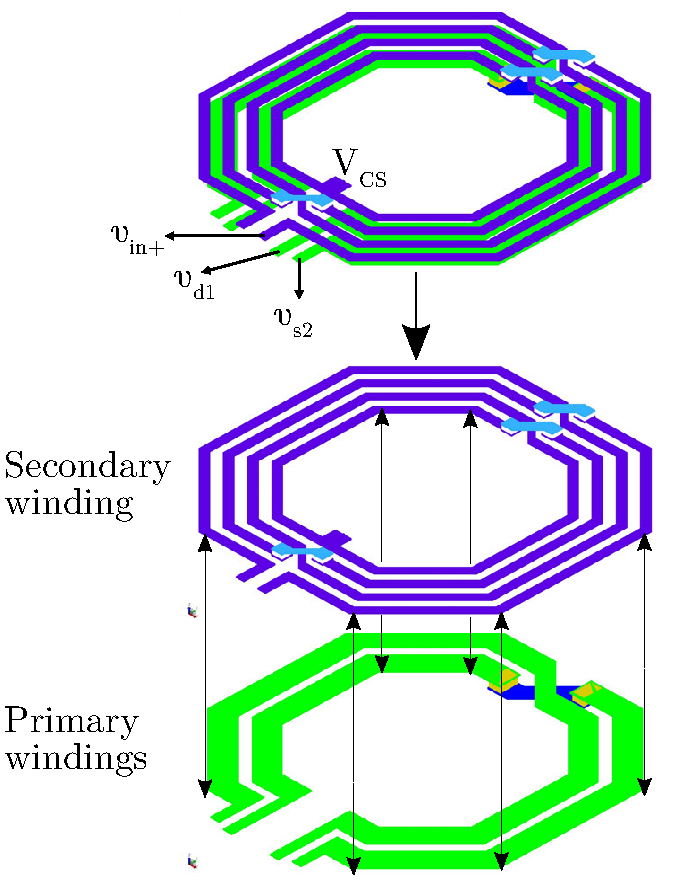
\includegraphics[width=0.6\linewidth]{assets/FD-SOI/Sub_6GHz_TRX_assets/LNA_inductors.pdf}
				\caption{Three-dimensional representation of the transformer used in the LNA of figure \ref{fig:FDSOI:TRX:LNA}. Figure taken from \cite{FDSOI2}.}
				\label{fig:FDSOI:LNA:transformers}
			\end{figure}

		Figure \ref{fig:FDSOI:TRX:IC} shows a photograph of the fabricated integrated circuit. The ratios of the LNA's input-transistors and the ratios of the output-transistors are $S_{1x}$ and $S_{2x}$, respectively.
		\begin{align*}
			&S_{1x}=\frac{W_{1x}}{L_{1x}}=\frac{0.9\unit{\milli\meter}}{28\unit{\nano\meter}}\approxeq 32,142.\overline{857\ 142}\\
			&S_{2x}=\frac{W_{2x}}{L_{2x}}=\frac{0.8\unit{\milli\meter}}{150\unit{\nano\meter}}\approxeq 5,333.\overline{3}
		\end{align*}
		\begin{figure}[h!]
			\centering
			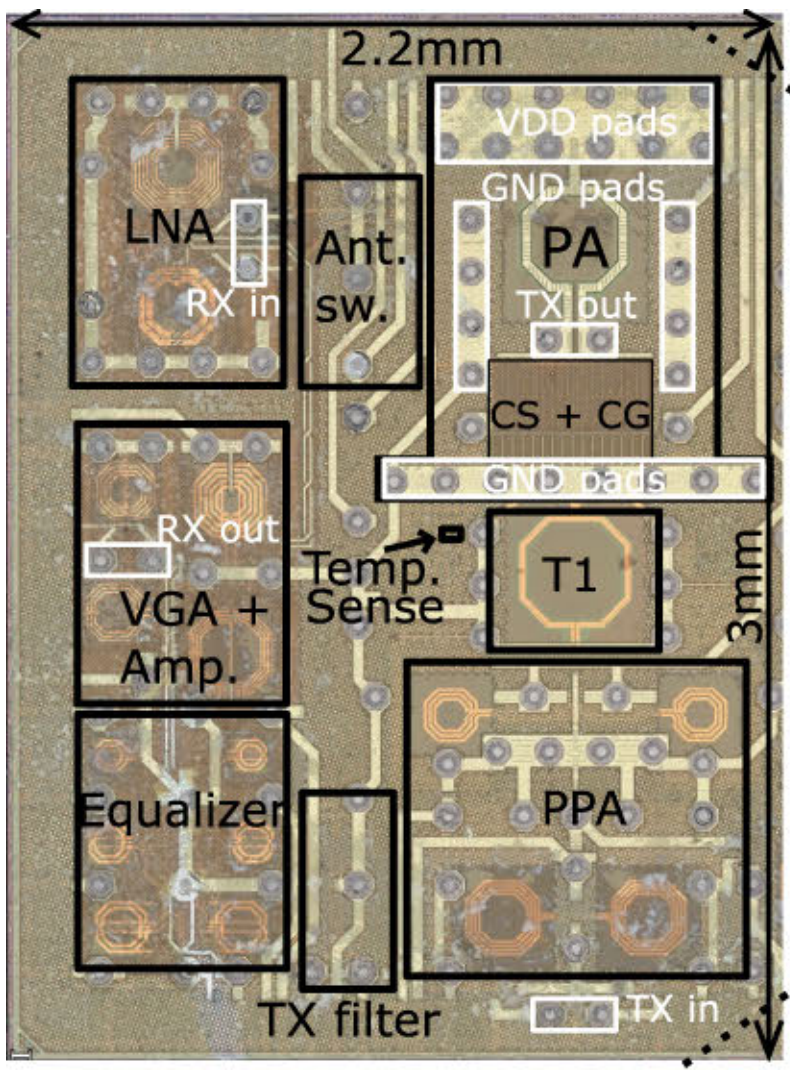
\includegraphics[width=0.7\linewidth]{assets/FD-SOI/Sub_6GHz_TRX_assets/IC.png}
			\caption{Photograph of the fabricated IC \cite{FDSOI2}.}
			\label{fig:FDSOI:TRX:IC}
		\end{figure}

		\begin{figure*}[ht!]
			\centering
			% \resizebox{1.5\linewidth}{!}{
\begin{tikzpicture}
    \node[shape=rectangle, fill={rgb,255:red,239;green,209;blue,209}, minimum width=6cm, minimum height=2.75cm] at (5, 3.125){};
    \node[shape=rectangle, fill={rgb,255:red,239;green,209;blue,209}, minimum width=6cm, minimum height=2.75cm] at (-5, 3.125){};
    \draw (-1, 5.25) to[cute inductor, l_=$L_g$] (-1, 6.25);
    \node[vcc, rotate=90](N1) at (-1.21, 5.75){} node[anchor=east] at ([xshift=0.12cm]N1.text){$V_{\symup{CS}}$};
    \node[circ, xscale=-1, yscale=-1] at (-1.21, 5.75){};
    \draw (1, 5.25) -- (1, 5);
    \node[circ] at (-1, 5){};
    \node[circ] at (1, 5){};
    \draw[-latex] (0.25, 5) -- (-0.25, 5);
    \draw (-1, 5) -- (-0.5, 5);
    \draw (0.5, 5) -- (1, 5);
    \node[ocirc] at (-0.5, 5){};
    \node[ocirc] at (0.5, 5){};
    \draw[-latex] (-0.667, 5) -- (-0.833, 5);
    \draw[-latex] (0.833, 5) -- (0.667, 5);
    \node[shape=rectangle, minimum width=0.465cm, minimum height=0.465cm](N2) at (-0.714, 4.75){} node[anchor=center] at (N2.text){$i_{\symup{in}}$};
    \node[shape=rectangle, minimum width=0.465cm, minimum height=0.436cm](N3) at (0.714, 4.765){} node[anchor=center] at (N3.text){$i_{\symup{in}}$};
    \draw[-latex] (-4.75, 5.25) -- (-4.75, 7.75);
    \node[shape=rectangle, minimum width=0.715cm, minimum height=0.715cm](N4) at (-4.375, 6.5){} node[anchor=center] at (N4.text){$v_{L_{dl}}$};
    \draw (-6, 6.5) to[cute inductor, l_={$L_{dl}$}] (-6, 5.25);
    \draw (-6, 7.75) to[american controlled voltage source, mirror, l_={$s\left( M_1 i_{L_g} - M_2 i_{dr}\right)$}] (-6, 6.75);
    \draw[dash pattern={on 1.6pt off 1.6pt}] (-6, 8) -- (-4.75, 8);
    \node[ocirc] at (-4.75, 8){};
    \draw[dash pattern={on 1.6pt off 1.6pt}] (-6, 5) -- (-4.75, 5);
    \node[ocirc] at (-4.75, 5){};
    \node[circ] at (-6, 8){};
    \node[circ] at (-6, 5){};
    \draw[-latex] (4.75, 5.25) -- (4.75, 7.75);
    \node[shape=rectangle, minimum width=0.715cm, minimum height=0.715cm](N5) at (4.375, 6.5){} node[anchor=center] at (N5.text){$v_{L_{dr}}$};
    \draw[dash pattern={on 1.6pt off 1.6pt}] (4.75, 5) -- (6, 5);
    \draw[dash pattern={on 1.6pt off 1.6pt}] (4.75, 8) -- (6, 8);
    \node[ocirc] at (4.75, 5){};
    \node[shape=rectangle, minimum width=0.715cm, minimum height=0.715cm](N6) at (5.625, 8.5){} node[anchor=center] at (N6.text){$i_{dr}$};
    \draw (6, 6.5) to[cute inductor, mirror, l={$L_{dr}$}] (6, 5.25);
    \node[circ] at (6, 8){};
    \node[circ] at (6, 5){};
    \draw (1, 6.25) to[american controlled voltage source, l={$s M_1 \left(i_{dl} - i_{dr}\right)$}] (1, 5.25);
    \draw (-6, 9) -- (-6, 7.75);
    \draw (-6, 5.25) -- (-6, 4);
    \draw (-6, 6.75) -- (-6, 6.5);
    \node[ocirc] at (-6, 9){};
    \draw[-latex] (-6, 8.75) -- (-6, 8.25);
    \node[shape=rectangle, minimum width=0.715cm, minimum height=0.715cm](N7) at (-5.625, 8.5){} node[anchor=center] at (N7.text){$i_{dl}$};
    \draw (6, 5.25) -- (6, 4);
    \draw (6, 7.75) to[american controlled voltage source, mirror, l={$s\left( -M_1 i_{L_g} - M_2 i_{dl}\right)$}] (6, 6.75);
    \draw (6, 9) -| (6, 7.75);
    \draw[-latex] (6, 8.75) -- (6, 8.25);
    \node[ocirc] at (6, 9){};
    \node[ocirc] at (4.75, 8){};
    \draw (6, 6.75) -| (6, 6.5);
    \draw (-6, 4) to[american controlled current source, l_={$g_m^{\text{\tiny{(11)}}} v_{gs}^{\text{\tiny{(11)}}}$}] (-6, 3);
    \draw (-3.5, 4) to[capacitor, l_={$C_{gs}^{\text{\tiny{(11)}}}$}] (-3.5, 3);
    \draw (-6, 3) -| (-6, 2.5) -| (-3.5, 3);
    \node[shape=rectangle, minimum width=0.715cm, minimum height=0.715cm](N8) at (-2.625, 3.5){} node[anchor=center] at (N8.text){$v_{gs}^{\text{\tiny{(11)}}}$};
    \draw[-latex] (-3, 3) -- (-3, 4);
    \draw (-3.5, 4) -| (-3.5, 5) -- (-1, 5);
    \draw (6, 4) to[american controlled current source, l={$g_m^{\text{\tiny{(12)}}} v_{gs}^{\text{\tiny{(12)}}}$}] (6, 3);
    \draw (3.5, 4) to[capacitor, l={$C_{gs}^{\text{\tiny{(12)}}}$}] (3.5, 3);
    \node[shape=rectangle, minimum width=0.715cm, minimum height=0.715cm](N9) at (2.625, 3.5){} node[anchor=center] at (N9.text){$v_{gs}^{\text{\tiny{(12)}}}$};
    \draw[-latex] (3, 3) -- (3, 4);
    \draw (3.5, 3) -| (3.5, 2.5) -| (6, 3);
    \draw (1, 5) -- (3.5, 5) -- (3.5, 4);
    \draw (-1, 5.25) -| (-1, 5);
    \draw (-1, 6.25) -| (-1, 6.5) -| (1, 6.25);
    \node[shape=rectangle, minimum width=0.715cm, minimum height=0.465cm](N10) at (0, 4.75){} node[anchor=center] at (N10.text){$v_{\symup{in}}$};
    \draw (-4.75, 2.5) -| (-4.75, 2) -| (4.75, 2.5);
    \node[circ] at (-4.75, 2.5){};
    \node[circ] at (0, 2){};
    \node[circ] at (4.75, 2.5){};
    \draw (0, 2) to[cute inductor, l={$L_{\symup{deg}}$}] (0, 0.5);
    \node[tlground] at (0, 0.5){};
    \node[shape=rectangle, minimum width=0.465cm, minimum height=0.465cm](N11) at (-3.75, 4.25){} node[anchor=center] at (N11.text){$\symup{G}$};
    \node[shape=rectangle, minimum width=0.465cm, minimum height=0.465cm](N12) at (3.75, 4.25){} node[anchor=center] at (N12.text){$\symup{G}$};
    \node[shape=rectangle, minimum width=0.465cm, minimum height=0.465cm](N13) at (-5.75, 4.25){} node[anchor=center] at (N13.text){$\symup{D}$};
    \node[shape=rectangle, minimum width=0.465cm, minimum height=0.465cm](N14) at (5.75, 4.25){} node[anchor=center] at (N14.text){$\symup{D}$};
    \node[shape=rectangle, minimum width=0.465cm, minimum height=0.465cm](N15) at (5, 2.25){} node[anchor=center] at (N15.text){$\symup{S}$};
    \node[shape=rectangle, minimum width=0.465cm, minimum height=0.465cm](N16) at (-5, 2.25){} node[anchor=center] at (N16.text){$\symup{S}$};
    \node[shape=rectangle, minimum width=0.465cm, minimum height=0.465cm](N17) at (0, 6.75){} node[anchor=center] at (N17.text){$i_{L_{g}}$};
    \draw[-latex] (0.25, 6.5) -- (-0.25, 6.5);
\end{tikzpicture}
% }
			\caption{Small signal equivalent of figure \ref{fig:FDSOI:TRX:LNA} with reactive series-shunt feedback. Transistors $\symup{M_{21}}$ and $\symup{M_{22}}$ are omitted from the model for clarity.}
			\label{fig:FDSOI:TRX:LNA_REACTIVE_FEEDBACK}
		\end{figure*}